%%%%%%%%%%%%%%%%%%%%%%%%%%%%%%%%%%%%%%%%%%%%%%%%%%%%%%%%%% 
\section{実行実験}\label{chap:experiment}
%%%%%%%%%%%%%%%%%%%%%%%%%%%%%%%%%%%%%%%%%%%%%%%%%%%%%%%%%% 

本章では,前章で提案した3つの符号化
\textsf{undirected},\textsf{directed},\textsf{acyclicity}
の性能を評価するために実行実験を行った.
%
実験に使用したベンチマーク問題集(計495問)は,以下の通りである.
\begin{itemize}
\item \textsf{color04} (計127問)\\
  グラフ彩色問題の国際競技会
  COLOR02/03/04~\footnote{\url{https://mat.tepper.cmu.edu/COLOR02/}}
  で使用された問題インスタンス.
\item \textsf{complete} (計15問)\\
  SATソルバーを用いた既存研究~\cite{soh14:jelia2014}で提供された
  完全グラフのインスタンス~\footnote{\url{https://tsoh.org/scarab/jelia2014/}}.
\item \textsf{knight} (計11問)\\
%  \cite{DBLP:conf/sat/EenS03}で用いられた
  $N\times N$の騎士巡回問題(Knight's Tour)のインスタンス.\\
  $N=8,12,20,30,40,50,60,70,80,90,100$の11通り.
\item \textsf{tsplib} (9問)\\
  巡回セールスマン問題のポータルサイトTSPLIBに公開されている
  インスタンス\footnote{\url{http://comopt.ifi.uni-heidelberg.de/software/TSPLIB95/hcp/}}.
\item \textsf{grid} (12問)\\
  $N$次の正方グリッドグラフのインスタンス($6\leq N\leq 17$).
\item \textsf{random} (320問)\\
  SATソルバーを用いた既存研究~\cite{soh14:jelia2014}で提供された
  ランダムグラフのインスタンス~\footnotemark[1].
\item \textsf{usmap} (1問)\\
  図~\ref{fig:USmap}に示されたグラフ.
  D.~E~.Knuth の教科書
  The Art of Computer Programming~\cite{Knuth:TAOCP:SAT}
  に記載されている最短ハミルトン路問題の例.
\end{itemize}

使用した ASP システムは{\clingo}のバージョン5.4.0である.
実験環境は,Mac mini Intel Corei7 3.2GHz 64GBメモリである.

%%%%%%%%%%%%%%%%%%%%%%%%%%%%%%%%%%%%%%%%%%%%%%%%%%%%%%%%%%
\subsection{ハミルトン閉路問題の実験結果}
%%%%%%%%%%%%%%%%%%%%%%%%%%%%%%%%%%%%%%%%%%%%%%%%%%%%%%%%%%

%%%%%%%%%%%%%%%%%%%%%%%%%%%%%%%%%%%%%%%%%%%%%%%
\begin{table}[t]\scriptsize
  \centering
  %\tabcolsep = 0.8mm
  \renewcommand{\arraystretch}{1.2}
  \begin{tabular}{lr|rrr}
    問題サイズ & 問題数 & \textsf{undirected} & \textsf{directed} & \textsf{acyclicity}\\
   \hline
    $\:\:\:\:\:\,\, 0 \leq |V| < 1000$     & 171   & 156   & \alert{171}   & 156  \\ %
    $1000 \leq |V| < 2000$  & 165   & 120   & \alert{159}   & 121  \\
    $2000 \leq |V| < 3000$  & 177   & 125   & \alert{163}   & 80   \\
    $3000 \leq |V| < 4000$  & 185   & 104   & \alert{147}   & 48   \\
    $4000 \leq |V| < 5000$  & 128   & 92    & \alert{106}   & 30   \\
    $5000 \leq |V| < 6000$  & 80    & 63    & \alert{70}    & 21   \\
    $6000 \leq |V| < 7000$  & 55    & 39    & \alert{41}    & 20   \\
    $7000 \leq |V| < 8000$  & 28    & 12    & \alert{15}    & 4    \\
    $8000 \leq |V| < 9000$  & 10    & 2     & \alert{5}     & 1    \\
    $9000 \leq |V| < 10000$  & 2     & \alert{2}     & \alert{2}     & 1    \\
   \hline
    合計 & 1001 & 715   & \alert{879}   & 482  
  \end{tabular}
  \vskip .5em
%  \caption{ハミルトン閉路問題: 解けた問題数}
  \label{sat_table}
\end{table}
%label{sat_table}
%%%%%%%%%%%%%%%%%%%%%%%%%%%%%%%%%%%%%%%%%%%%%%%

%%%%%%%%%%%%%%%%%%%%%%%%%%%%%%%%%%%%%%%%%%%%%%%
\begin{figure}[tb]
\begin{center}
  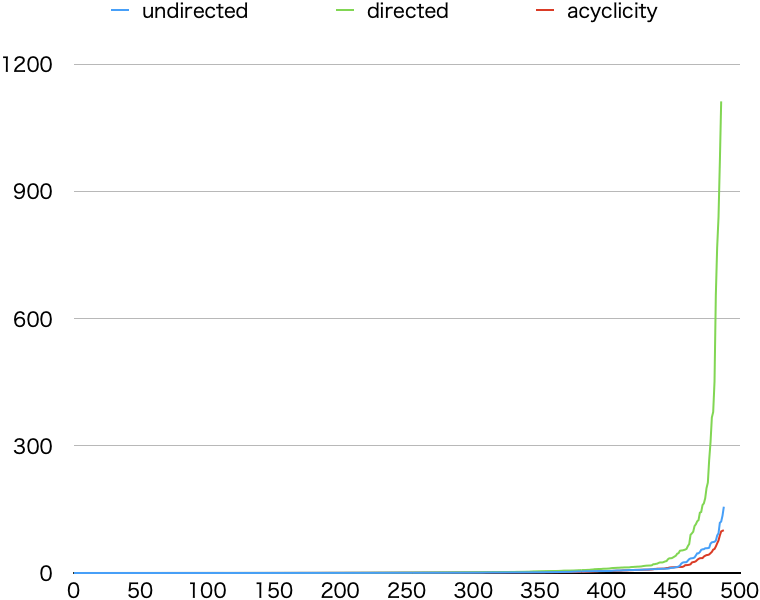
\includegraphics[width=0.8\linewidth]{fig/cactus.png}
\caption{ハミルトン閉路問題: カクタスプロット (\textsf{SAT+UNSAT})}
\label{cactus}
\end{center}
\end{figure}
%%%%%%%%%%%%%%%%%%%%%%%%%%%%%%%%%%%%%%%%%%%%%%%

%%%%%%%%%%%%%%%%%%%%%%%%%%%%%%%%%%%%%%%%%%%%%%%
\begin{figure}[tb]
\begin{center}
  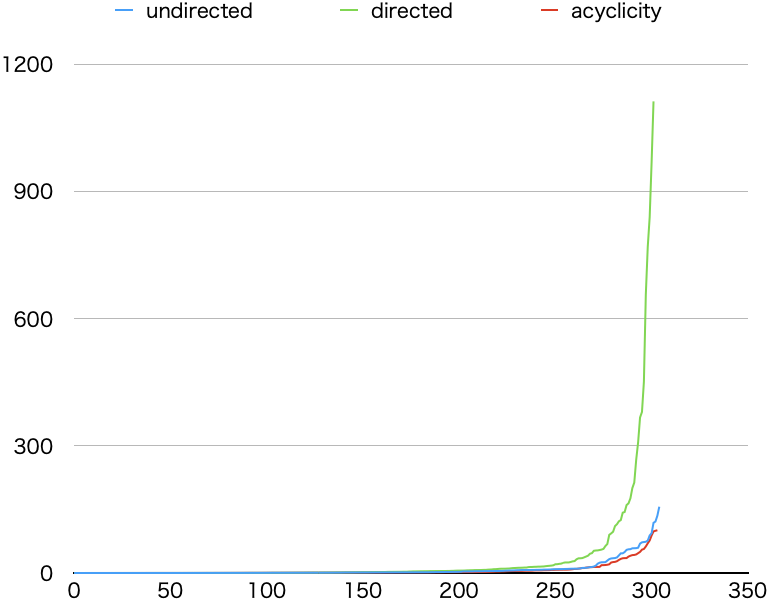
\includegraphics[width=0.8\linewidth]{fig/cactussat.png}
\caption{ハミルトン閉路問題: カクタスプロット (\textsf{SAT})}
\label{cactussat}
\end{center}
\end{figure}
%%%%%%%%%%%%%%%%%%%%%%%%%%%%%%%%%%%%%%%%%%%%%%%

%%%%%%%%%%%%%%%%%%%%%%%%%%%%%%%%%%%%%%%%%%%%%%%
\begin{figure}[tb]
\begin{center}
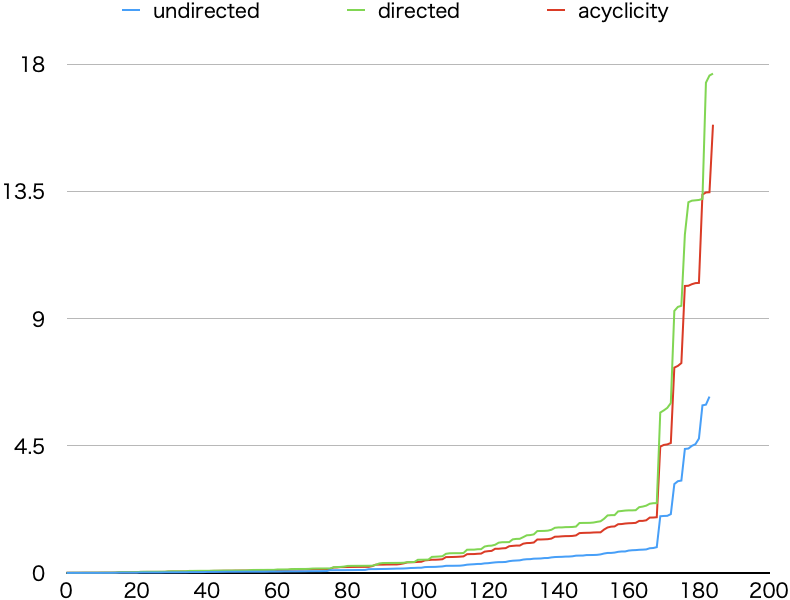
\includegraphics[width=0.8\linewidth]{fig/cactusunsat.png}
\caption{ハミルトン閉路問題: カクタスプロット (\textsf{UNSAT})}
\label{cactusunsat}
\end{center}
\end{figure}
%%%%%%%%%%%%%%%%%%%%%%%%%%%%%%%%%%%%%%%%%%%%%%%

%--
本節では,ハミルトン閉路問題の実験結果について述べる.
{\clingo}のオプションは\textit{trendy}を使用し,一問あたりの時間制限を30分とした.
ベンチマーク問題は,
\textsf{color04},
\textsf{complete},
\textsf{knight},
\textsf{tsplib},
\textsf{grid},
\textsf{random}の合計494問である.

%--
表~\ref{sat_table}に,各符号化で解けた問題数を示す.
左から,問題の種類,問題数,各符号化で解けた問題数を,
\textsf{SAT},\textsf{UNSAT},\textsf{SAT+UNSAT}
毎に示している.
%
\textsf{SAT+UNSAT}の解けた問題数は,
\textsf{undirected}符号化が490問,
\textsf{directed}符号化が488問,
\textsf{acyclicity}符号化が490問であり,
\textsf{undirected}と\textsf{acyclicity}が,
\textsf{directed}よりも2問多く解いた.
図~\ref{cactus}に,\textsf{SAT+UNSAT}のカクタスプロットを示す.
縦軸は問題を解くのに要した CPU 時間,横軸は解けた問題数を表す.
グラフが右によるほど多くの問題を解けたことを示し,
下によるほどより速く解けたことを示す.
図~\ref{cactus}より,\textsf{acyclicity}符号化は,解けた問題数が同じ
\textsf{undirected}符号化と比較して,僅かではあるが,より高速に問題を
解いていることが確認できた.

\textsf{SAT}のみの場合は,
\textsf{undirected}符号化が305問,
\textsf{directed}符号化が302問,
\textsf{acyclicity}符号化が304問であり,
\textsf{undirected}が,最も多くの問題を解いた.
\textsf{SAT}のみの場合のカクタスプロットを図~\ref{cactussat}に示す.
\textsf{directed}符号化が,
\textsf{undirected}および\textsf{acyclicity}と比較して,
性能が劣ることが確認できた.
%
\textsf{UNSAT}のみの場合は,
\textsf{undirected}符号化が185問,
\textsf{directed}符号化が186問,
\textsf{acyclicity}符号化が186問であり,
\textsf{directed}と\textsf{acyclicity}符号化が,
\textsf{undirected}より1問多く解いている.
\textsf{UNSAT}のみの場合のカクタスプロットを図~\ref{cactusunsat}に示す.
解けた問題数が同じであった\textsf{directed}と\textsf{acyclicity}を比較
すると,僅かではあるが,\textsf{acyclicity}がより高速に問題を解いてい
ることが確認できた.

%--
%% これらの結果から,
%% \textsf{SAT}な問題に対しては,解けた問題数と解くのに要したCPU時間
%% のどちらにおいても\textsf{acyclicity}符号化が優秀であったことがわかる.
%% 一方で,\textsf{UNSAT}な問題に対しては,
%% 解けた問題数では\textsf{directed}符号化と\textsf{acyclicity}符号化が,
%% 解くのに要したCPU時間では\textsf{undirected}符号化がそれぞれ優秀であったことがわかる.

% %--
% また,表~\ref{sat_table}より,
% \textsf{SAT+UNSAT}の問題数については,
% \textsf{undirected}符号化と\textsf{acyclicity}符号化は同数だった.
% しかし,その内訳には差があった.
% 結果に差があった問題は,\textsf{3-FullIns\_5}と\textsf{grid12}で,
% それぞれ\textsf{color04}の\textsf{SAT}と,
% \textsf{grid}の\textsf{UNSAT}に属する.
% \textsf{3-FullIns\_5}は\textsf{undirected}に解けて
% \textsf{acyclicity}に解けなかった.
% 一方で,\textsf{grid12}は,\textsf{acyclicity}に解けて
% \textsf{undirected}に解けなかった.

% \textsf{3-FullIns\_5}は\textsf{SAT}であったことから,
% \textsf{undirected}符号化は\textsf{3-FullIns\_5}でハミルトン閉路を
% 偶然速く見つけられたと考える.
% %% \textsf{color04}の他の問題を見ても,
% %% \textsf{undirected}符号化が優秀であることを示してはいない.
% %% 変数の数や制約の数も少なくない.
% \textsf{grid12}については,変数の数や制約の数において,
% \textsf{acyclicity}符号化が少ない値を示していたため,
% 要するCPUtimeを短縮できたと考える.

%% \textsf{grid12}は,\textsf{UNSAT}の問題に限定すれば
%% 要したCPU時間において優秀だった\textsf{undirected}符号化にのみ
%% 解けていなかった.
%% この問題の他にも,\textsf{grid}かつ\textsf{UNSAT}な問題を
%% 確認した.
%% \textsf{undirected}符号化がどの問題でも,
%% もっとも多く時間を要していた.
%% \textsf{undirected}符号化は\textsf{UNSAT}な\textsf{grid}問題が
%% 苦手であると考える.

%%%%%%%%%%%%%%%%%%%%%%%%%%%%%%%%%%%%%%%%%%%%%%%%%%%%%%%%%%
\subsection{最短ハミルトン閉路問題}
%%%%%%%%%%%%%%%%%%%%%%%%%%%%%%%%%%%%%%%%%%%%%%%%%%%%%%%%%%

%%%%%%%%%%%%%%%%%%%%%%%%%%%%%%%%%%%%%%%%%%%%%%%
\begin{table}[htbp]
  \caption{実験結果2-1:trendy}
  \label{min_table_tr}
  \centering
  \begin{tabular}{|l|rrr|}
    \hline
    Instance&undirected&directed&acyclicity \\
    \hline
    grid5&50,656*&50,656*&50,656* \\
    grid6&68,656*&68,656*&68,656* \\
    grid7&91,822*&91,822*&91,822* \\
grid8&113,250&\textcolor{red}{112,916}&113,277 \\
grid9&\textcolor{red}{142,502}&143,326&143,660 \\
grid10rc&\textcolor{red}{172,703}&174,866&175,999 \\
grid11&\textcolor{red}{200,399}&204,456&200,638 \\
grid12&\textcolor{red}{231,278}&239,275&232,012 \\
grid13&\textcolor{red}{276,692}&276,926&276,899 \\
grid14&317,617&\textcolor{red}{317,144}&317,676 \\
grid15&\textcolor{red}{375,906}&376,809&376,210 \\
grid16&421,249&\textcolor{red}{419,737}&423,753 \\
US48&11,698*&11,698*&11,698* \\
    \hline
  \end{tabular}
\end{table}
%\label{min_table_tr}
%%%%%%%%%%%%%%%%%%%%%%%%%%%%%%%%%%%%%%%%%%%%%%%

%--
本節では,最短ハミルトン閉路問題の実験結果について述べる.
{\clingo}のオプションは\textit{trendy}を使用し,
一問あたりの時間制限を3時間とした.
ベンチマーク問題は,\textsf{grid}と\textsf{usmap}の合計13問である.

%--
表\ref{min_table_tr}に,各符号化で得られた最適値と最良値を示す.
各問題毎に,最も良かった値を赤字で示している.
*マークは,最適値を表している.
最適値と最良値の数は,
\textsf{undirected}符号化が10問,
\textsf{directed}符号化が7問,
\textsf{acyclicity}符号化が4問であり,
\textsf{undirected}符号化の優位性が確認できた.


%%%%%%%%%%%%%%%%%%%%%%%%%%%%%%%%%%%%%%%%%%%%%%%%%%%%%%%%%%
\subsection{コスト制約付きハミルトン路問題}
%%%%%%%%%%%%%%%%%%%%%%%%%%%%%%%%%%%%%%%%%%%%%%%%%%%%%%%%%%

%%%%%%%%%%%%%%%%%%%%%%%%%%%%%%%%%%%%%%%%%%%%%%%
\begin{table*}[tb]\footnotesize
  \tabcolsep = 2mm
  %\renewcommand{\arraystretch}{1.0}
  \vskip .5em
  \centering
  \begin{tabular}{lr|rrr}
    \hline
    閾値(倍率)    &	解の総数 & \textsf{undirected} & \textsf{directed} & \textsf{acyclicity} \\
    \hline
    11698(1.00)   &	1      &\textbf{2.979} & 7.531 & 4.586	\\
    11814(1.01)   &	8      &5.587  & 15.322	& \textbf{5.250}	\\
    11931(1.02)   &	28     &\textbf{3.243}& 18.600	& 3.578	\\
    12282(1.05)   &	388    &10.003&19.818	& \textbf{6.296}	\\
    12867(1.10)   &	16,180  &16.548& 28.555	& \textbf{9.764}\\
    14037(1.20)   &	939,209 &48.262       &40.717	& \textbf{26.837}\\
    15207(1.30)   &	4,525,541&88.172      &55.276	& \textbf{42.037}\\
    16377(1.40)   &	6,702,964&99.154       &47.647	& \textbf{40.640}	\\
    17547(1.50)   &	6,876,526&95.390       &45.265	& \textbf{38.411}	\\
    18716(1.60)   &	6,876,928&98.937       &49.138	& \textbf{40.748}	\\
    \hline
    平均CPU時間 &   & 46.8275 & 32.7869  & \textbf{21.8147}\\\hline
%    Best    &   & 2 & 0 & \textbf{8} \\ \hline
  \end{tabular}
  \vskip .5em
  \caption{コスト制約付きハミルトン路問題: 解の全列挙に要した CPU 時間}
  \label{cost_table}
\end{table*}
%\label{cost_table}
%%%%%%%%%%%%%%%%%%%%%%%%%%%%%%%%%%%%%%%%%%%%%%%

%--
本節では,第~\ref{chap:background}章でも説明した
コスト制約付きハミルトン路問題(全列挙)の実験結果について述べる.
{\clingo}のオプションは\textit{crafty}を使用し,
一問あたりの時間制限を3時間とした.
ベンチマーク問題は,D.~E~.Knuth の教科書
The Art of Computer Programming~\cite{Knuth:TAOCP:SAT}
に記載されているグラフを使用した(図~\ref{fig:USmap}参照).
このグラフは,米国本土48州の隣接関係を表しており,
頂点数は48,辺の数は105である.
この問題の最短距離は 11698 である(表~\ref{min_table_tr}参照).
今回の実験では,
コスト制約を最短距離のN倍以下
($N=1.00,1.01,1.02,1.05,1.1,1.2,1.3,1.4,1.5,1.6$)として,解の全列挙を
行った.

%--
表~\ref{cost_table}に,各符号化が解の全列挙に要した CPU 時間を示す.
表の1列目はコスト制約の閾値と最短距離からの倍率,2列目は解の総数を表している.
各閾値毎に,最も良かった値を赤字で示している.
表より,
\textsf{acyclicity}符号化が,他の符号化と比較して,より多くの問題を
高速に解いていることがわかる.また,平均CPU時間も最も短い.
%%%%%%%%%%%%%%%%%%%%%%%%%%%%%%%%%%%%%%%%%%%%%%%%%%%%%%%%%%

%%% Local Variables:
%%% mode: latex
%%% TeX-master: "paper"
%%% End:
